\chapter{Rozšíření HEAppE pro lokální výpočty}
Jedním z hlavních cílů této práce je navrhnout a implementovat rozšíření HEAppE Middleware o možnost lokálních výpočtů, tedy umožnit uživateli nasimulovat spouštění úloh lokálně počítači s využití rozhraní HEAppE, a to bez nutnosti spojení se superpočítačem. Výhodou tohoto rozšíření je především možnost nezávislé přípravy specifikace úlohy a vyzkoušení práce s HEAppE.

Jelikož je systém HEAppE Middleware zpravidla nasazován za pomocí technologie Docker na servery superpočítačového centra, tak je možné tento způsob pohodlně replikovat i na uživatelském počítači. Technologie Docker je možné nainstalovat jako službu na počítače s operačními systémy Windows, Mac i Linux.

Cílem tohoto rozšíření je co možná největší udržení systémové nezávislosti. Mělo by simulovat HEAppE komunikaci s clustery. Na straně simulovaného HPC clusteru v prostředí uživatelského počítače by mělo být dosaženo co nejpodobnější chování plánovače, jako je tomu na skutečných výpočetních clusterech.

\section{Návrh řešení}
Toto rozšíření bylo navrženo s ohledem na platformní nezávislost a využití stávajících principů, na kterých stojí HEAppE Middleware.

Jelikož je HEAppE postaven na kontejnerizační technologii Docker, tak bylo navrženo, aby samotný virtuální HPC cluster byl spouštěn také jako kontejner. Pro uživatele by mělo být poměrně jednoduché řešení, neboť by šlo jen o malou úpravu stávající Docker konfigurace (přidání vazby na kontejner) a přidání záznamu virtuálního clusteru do databáze (popř. upravení tzv. seedu) – přesně tak, jak je tomu i při přidávání specifikace skutečného HPC clusteru.

Celá koncepce návrhu rozšíření je vyobrazena v následujícím diagramu.

\newpage
\begin{figure}
	\centering
	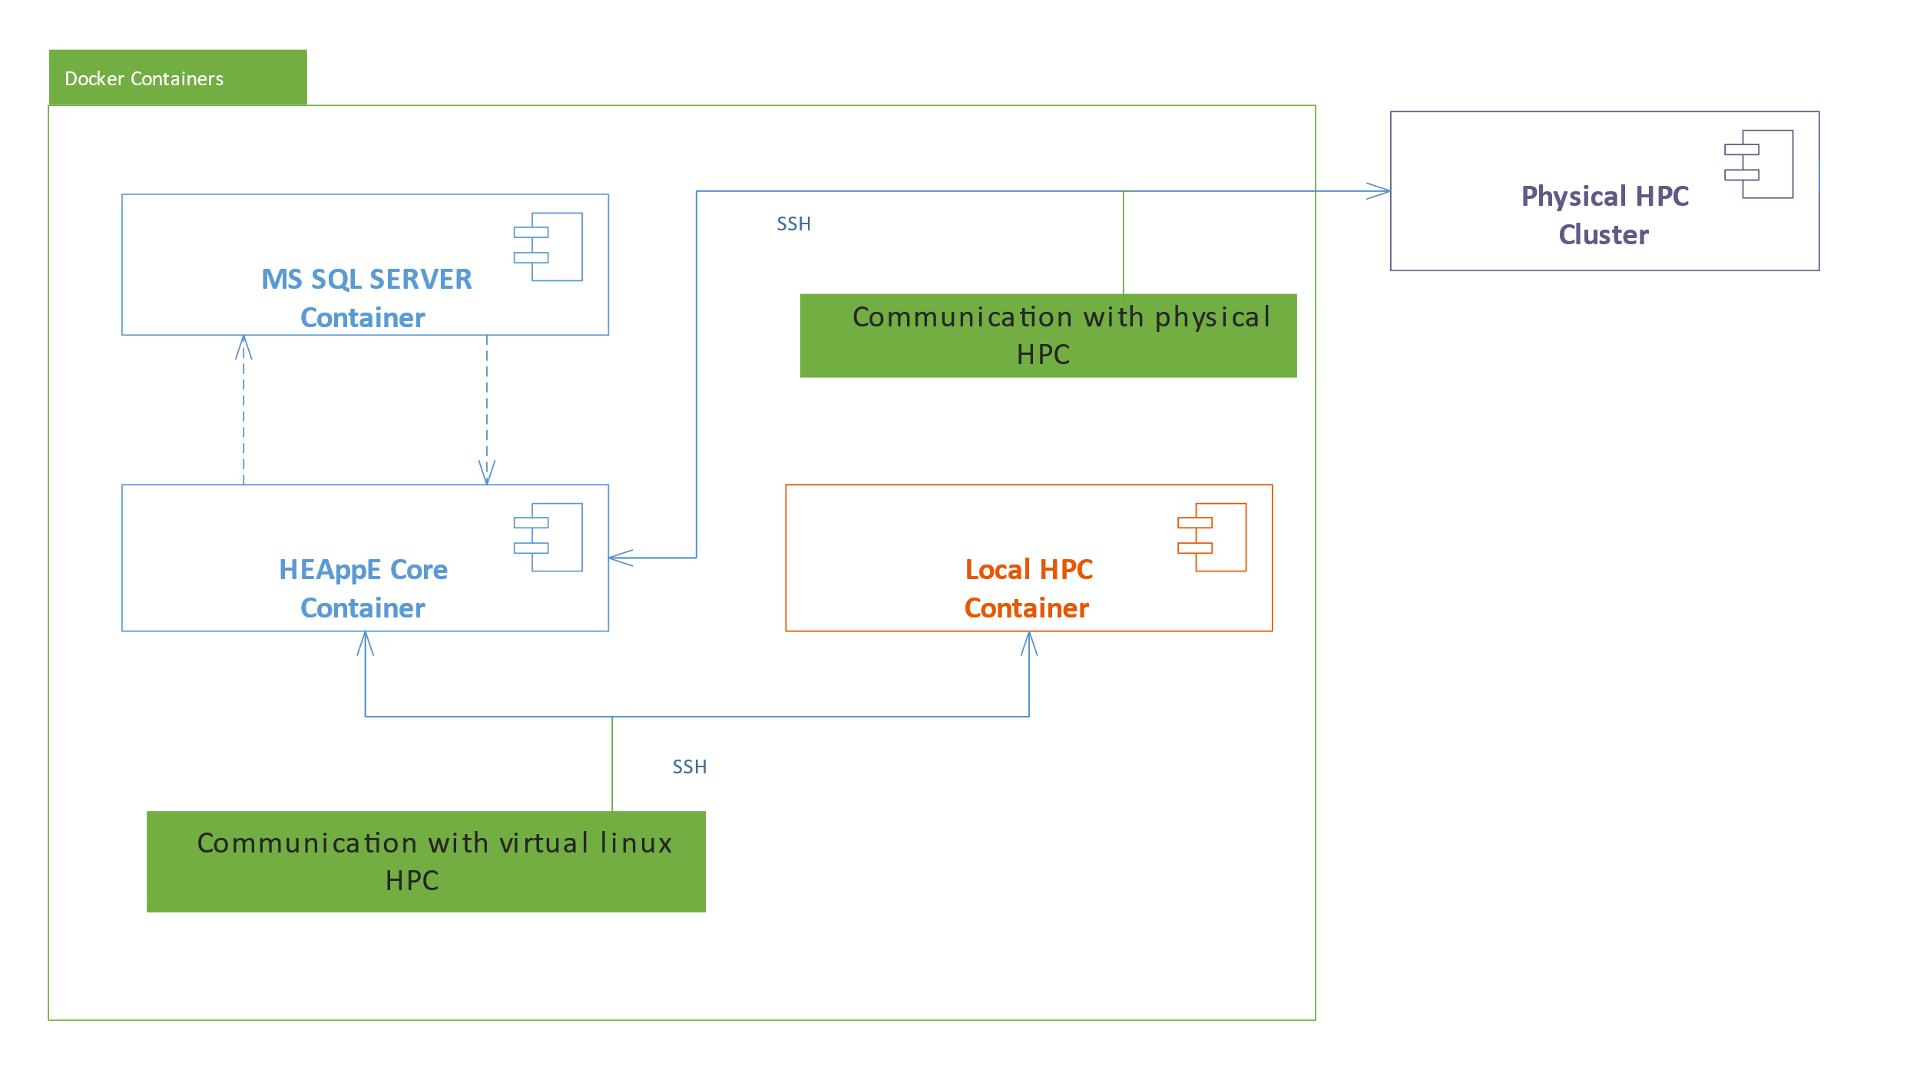
\includegraphics[width=1.0\textwidth]{Figures/local-hpc-clsuter-navrh.png}
	\caption{Návrh rozšíření o lokální HPC cluster}
	\label{fig:navrh-rozsireni-o-lokalni-hpc-clsuter}
\end{figure}

Lokální HPC Cluster je z technického hlediska spouštěná instance virtuálního stroje s OS Linux. K nasimulování chování plánovače, který je součástí superpočítače, bude v tomto případě využito několik skriptů, které se budou spouštěny na žádost HEAppE. HEAppE Middleware bude upraven minimálně, úpravy nebudou zasahovat do logiky užívání při spojení s plánovači na superpočítačích, a to i z důvodu možnosti zanesení chyby do stávajícího řešení. V systému HEAppE je několik vrstev, kterými se prochází od požadavku uživatele nad API, největší úpravy budou v poslední vrstvě – HpcConnectionFramework, kde bude přidán konektor (SchedulerAdapter) pro práci s lokálním virtuálním strojem simulující chování plánovače na superpočítači.

Vrstvy v HEAppE jsou tvořeny s ohledem na pozdější úpravy či přidávání dalších adaptérů apod. Je využíváno návrhového vzoru Abstract Factory (abstraktní továrna), k tomuto návrhovému vzoru bude přihlíženo při výše popsaných úpravách.

\section{Konfigurace virtuálního stroje}
Velkou výhodou použití Docker engine je snazší distribuce komponent systému. Pro jednotlivé kontejnery stačí vytvořit konfiguraci, popř. připravit obraz spouštěné služby. Kontejnery je pak možné spouštět dohromady, je mezi nimi možné vytvořit komunikační kanály. Právě tímto způsobem pak bude realizována simulovaná komunikace mezi HEAppE a virtuálním HPC clusterem.

Výhodu je také to, že do konfigurace je možné zanést aktuální stav virtuálního stroje, tak aby koncový uživatel měl vše připraveno. V případě této instance budou nastaveny komunikační porty, vytvořen uživatel v systému OS Linux, uloženy skripty pro simulování komunikace s plánovačem, nebo zde např. budou připraveny testovací SSH-RSA klíče a povolena komunikace mezi kontejnery.

Tato konfigurace nese označení dockerfile, jedná se o soupis kroků či povelů, které se stanou při spouštění kontejneru. Od stažení obrazu OS Linux, až po zpřístupnění komunikačního portu.

Následuje ukázka využívaného dockerfile pro instanci lokálního HPC clusteru.

\hfill \break
\lstinputlisting[language=Dockerfile,caption={dockerfile konfigurace pro virtuální stroj},breaklines=true]{SourceCodes/dockerfile}

\section{Komunikace mezi HEAppE a virtuálním HPC}
Ke komunikaci mezi HEAppE a skutečným superpočítačovým clusterem probíhá především prostřednictvím protokolu SSH. Komunikace je založena na principu klient-server (heappe-HPC). Prostřednictvím SSH HEAppE odesílá příkazy např. pro vytvoření, spouštění úlohy apod. Zpět dostává od plánovače data o provedení příkazu, vyžádaná data, popř. aktuální stav úlohy.

Obdobně byla navržena komunikace i mezi HEAppE a virtuálním strojem simulující chování plánovače superpočítačového clusteru. Komunikace taky probíhá prostřednictvím SSH s využitím autentizace, tak aby byla simulace co nejvěrohodnější.

\section{Data a stav úloh}
HEAppE je stavěno tak, že se na obou stranách (HEAppE i HPC) uchovávají data o prováděných úlohách. HEAppE si v době běhu úlohy na superpočítači cyklicky žádá o data. A postupně se takto obě databáze synchronizují. Data jsou poskytována pouze na vyžádání, nejedná se o sdílený datový prostor. Data jsou z HPC zasílána v předem známém formátu v textové podobě zpět při SSH komunikaci.

Obdobně je přistupováno k datům i v případě simulace HPC na lokálním virtuálním stroji. S ohledem na výkon a režii nejsou data na straně virtuálního HPC ukládána v databázi. V adresáři dané úlohy je sada souborů, obsahující data (stav, parametry) úlohy. Tato data se nachází v předem definované JSON\footnote{JSON neboli JavaScript Object Notation je formát využívaný pro výměnu dat. Formát je jednoduše čitelný i pro člověka.\cite{lJoeVuQg92zsjaAe}}  struktuře, jsou ukládána a aktualizována při běhu úlohy. Po vyžádání jsou data zaslána v JSON struktuře textově zpět na HEAppE.

Pro práci s JSON strukturami slouží ve virtuálním stroji parser\footnote{Parser je program či jeho část provádějící syntaktickou analýzu textu. Analýza textu je proces, při němž je zpracováván text za pomoci definovaných pravidel daného jazyka.\cite{uEN4MdNhBpkZmkHF}} jq\cite{qibOqajDMnKYNjXq}. Jedná se o program, který je schopen z JSON struktury získat data nebo je naopak aktualizovat či přidat a odebrat. Tento program je instalován při startování Docker kontejneru, žádost o instalaci se nachází v konfiguraci dockerfile.

\hfill \break
\begin{lstlisting}[caption={Příklad JSON struktury}]
{
   "SessionCode": "string",
   "CreatedJobInfoId": 0
}
\end{lstlisting}

\section{Implementace na straně HEAppE Middleware}
Jak už bylo zmíněno výše, HEAppE Middleware je stavěn na rozhraní .NET Core, vyvíjí se v jazyce C\#. Z hlediska pohledu architektury se jedná o vrstvený systém. Uživatelské požadavky na REST API jsou zachyceny ve stejnojmenné vrstvě (RestAPi). Z této vrstvy jsou vstupní data po úspěšné validaci předávána do servisní a BusinessLogic vrstvy, ve které se nachází primární aplikační logika. Na závěr se požadavek dostává do vrstvy HpcConnectionFramework.

Vrstva HpcConnectionFramework je místem, kde dochází ke komunikaci s výpočetními clustery. V této vrstvě je implementováno několik adaptérů, které jsou schopny pracovat s odlišnými typy plánovačů na superpočítačích. Adaptéry jsou voleny na základě specifikace úloh, HEAppE předem musí mít v databázi informace o používaných clusterech a plánovačích. Právě v tomto místě se také skrývá největší část implementace pro komunikaci s lokálním simulovaným výpočetním clusterem.

Samotná implementace výše popsaného řešení se skládá z adaptéru, ve kterém se nachází logika pro komunikaci s virtuálním strojem. V tomto místě jsou připravovány příkazy ke spouštění skriptů pro řízení úloh a zpracovávány odpovědi lokálního HPC. Důležitou součástí je také datový konvertor, jehož úkolem je mapovat získaná data z lokálního HPC v JSON formátu na objekty nebo jejich kolekce. S těmi objekty je pak dále v HEAppE pracováno již obvyklým způsobem, jako je tomu u komunikace se skutečnými HPC. Nedílnou součástí celého adaptéru jsou připravené DTO objekty, přesněji se jedná o objekty popisující stav prováděné úlohy (JobDTO a TaskDTO). Součástí JobDTO je kolekce objektů TaskDTO (návrhový vzor Composite).

DTO objekty s napamovanými daty jsou pak v nižších vrstvách využity pro aktualizaci stavu a časů jednotlivých spouštěných úloh.

\section{Implementace na straně virtuálního stroje}
Konfigurace již zmiňovaného virtuálního stroje s OS Linux je sepsána jako sekvence kroků pro spouštění v prostředí Docker. Součástí konfigurace je stažení obrazu OS Linux (Minideb) vytvoření uživatele pro práci, nastavení přístupových práv, nastavení domovského adresáře, instalace openssh serveru pro komunikaci nebo například instalace programu jq pro jednodušší práci s JSON strukturami.

Z důvodu možnosti jednoduché a rychlé úpravy byly pro řízení běhu simulovaného plánovače využity scripty psány ve skriptovacím jazyce BASH. Zmíněné skripty programátor může jednoduše číst, orientovat se v nich, a protože se jedná o interpretovaný jazyk, tak se programy napsané v BASHi spouštějí přímo bez nutnosti kompilace. Pro využití s Docker konfigurací tyto programy patří mezi nejlepší možné rychlé a jednoduché řešení. Celkově tato koncepce navazuje na stávávající řídící skripty, které HEAppE využívá na skutečných výpočetních clusterech pro zjednodušení komunikace.

Mezi tyto stávající využívané skripty patří například skript vytvářející pracovní adresář pro dané úlohy, přidávání či odebírání ssh klíčů nebo skript pro přesun dat.

Parametry jednotlivých skriptů, které jsou zasílány z HEAppE jsou enkódovány do formátu Base64, aby nedocházelo k nechtěným problémům v případě zasílaných nepovolených znaků. Na straně virtuálního i skutečného výpočetního clusteru jsou tyto parametry dekódovány a užívány v textové podobě dle zvolené logiky.



\hfill \break
\lstinputlisting[language={},identifierstyle=\color{black},caption={Příklad Base64 kódování}]{SourceCodes/base64-enc.txt}

Řídící skripty, které mají za úkol nasimulovat chování plánovače na superpočítač jsou tři. Jedná o skript, který spouští samotnou úlohu, získává aktuální stav úlohy nebo získává počet úloh na simulovaném clusteru. Všechny tyto podpůrné skripty pracují jen se soubory a adresáři, aby nedocházelo ke zbytečné zátěži (není použit DB server apod.). 

\subsection{Skript pro přípravu úlohy}
Tento skript po spuštění připraví specifikace a parametry úlohy do kořenového adresáře úlohy na simulovaném HPC clsuteru. JSON struktura s popisem úlohy je vložena do souboru .job\_info. Příkazy kódované v Base64 jsou uloženy do souboru .commands. S těmito soubory, přesněji s jejich obsahem pracující další skripty, které jsou popsány níže.


\subsection{Skript pro spouštění úlohy}
Skript věrohodně simuluje chování postupného spouštění jednotlivých úloh, ty se staví do fronty. Využívá program jq k úpravám JSON struktury celé úlohy, která je uložena v souboru adresáře úlohy. Skript pracuje následujícím způsobem:

\begin{enumerate}
	\item Načtení předaných parametrů pro spouštění (příkazy uložené v souboru .commands v kořenouvém adresáři dané úlohy)
	\item Rozdělení jobů na jednotlivé na sebe navazující tasky
	\item Zapsání aktuálního času do stavové struktury úlohy (soubor .job\_info v kořenouvém adresáři dané úlohy)
	\item Zapsání stavu R (running) a PID (process ID) do stavové struktury
	\item Správa jednotlivých tasků (s ohledem na jobArrays, závislosti)
	\begin{enumerate}
		\item Vstup do adresáře tasku
		\item Uložení dat do stavové struktury k danému tasku (stav, čas)
		\item Spuštění úlohy
		\item Uložení stavu a času po dokončení úlohy
	\end{enumerate}
	\item Vstup do adresáře jobu
	\item Zapsání stavu a časů daného jobu (agregace stavů tasků)
	\item Ukončení scriptu
\end{enumerate}

Aktualizace datové struktury pro ukládání stavů (v souboru .job\_info) je okamžitě propsána do souboru po každé úpravě z důvodu nemožnosti předvídání čtení aktuálního stavu prostřednictvím HEAppE. Data musí být v každém kroku aktuální.

\subsection{Skript pro získání stavové struktury úlohy}
Po vyžádání dat (spuštění skriptu s parametry úlohy) je přistoupeno do adresáře úlohy a na výstup skriptu jsou odeslána data v textové podobě (JSON). Tato data jsou pak přijata v HEAppE a jak již bylo výše popsáno, jsou namapována na DTO objekt, se kterým se dále pracuje a v posledním kroku dojde k synchronizaci dat s databází HEAppE.

\subsection{Skript pro získání počtu úloh}
Skript na výstupu vrací počet adresářů s úlohami, které byly prostřednictvím HEAppE a řídících skriptů vytvořeny. Tento skript je využíván zejména pro JobReporting funkcionality HEAppE. Výstupem je např. report s jednoduchou statistikou užívání daného clusteru.

\subsection{Skript pro ukončení aktuálně běžící úlohy}
Protože HEAppE podporuje ukončení aktuálně běžící úlohy na HPC clusteru, tak bylo nutné vytvořit skript i pro virtuální HPC cluster, který ukončí právě běžící proces, který reprezentuje spuštěný skript (task). Tento skript přečte uložené číslo procesu (PID) na lokálním stroji simulující chování HPC plánovače, které se nachází v souboru .job\_info a vyšle zprávu danému běžícímu procesu (příkaz kill). Následně jsou změněny stavy a časová razítka ve struktuře úlohy na virtuálním HPC clsuteru.

\section{Nutné kroky ke spuštění}
V případě, že chce uživatel využívat HEAppE s tímto rozšířením pro simulaci výpočtu na lokálním počítači, tak musí provést následující kroky.

\begin{enumerate}
	\item Získání konfigurace kontejneru pro simulaci HPC se všemi skripty a soubory (obsahuje konfiguraci dockerfile)
	\item Úprava docker konfigurace HEAppE pro spouštění kontejnetu lokálního clusteru (příklad níže)
	\item Přidání clusteru do výchozího stavu dat databáze (seed)
	\begin{enumerate}
	    \item Protože se bude jednat o kumunikaci mezi Docker kontainery, musí být atribut MasterNodeName, který se využívá jako Host při nastavování spojení na cluster, nastaven na hodnotu "host.docker.internal" – není možné využít adresu localhost ani 127.0.0.1
	    \item Musí být nastaveny údaje pro autentizaci (username, password, private key, key file)
	    \item Musí být vytvořen nový uzel s frontou, kterou uživatel bude využívat na virtuálním HPC
	    \item Atribut SchedulerType musí být nastaven na hodnotu 1, interně je v logice HEAppE tento typ plánovače využit při volbě adaptéru ve vrstvě HpcConnectionFramework
	\end{enumerate}
\end{enumerate}

\begin{lstlisting}[language=Dockerfile,caption={Docker konfigurace pro spouštění kontejnetu lokálního clusteru}]
localhpc:
    container_name: localhpc
    build: C:/path/to/LocalLinuxHPCclusterConf
    ports:
    - "49005:22"
\end{lstlisting}


Přesnější popis nutného nastavení s přesnými údaji je uvedeno v textovém souboru u samotné konfigurace kontejneru.

Bod č. 1 je možné nahradit za spuštění docker kontejneru lokálního clusteru zvlášť. Bez návaznosti na ostatní služby HEAppE.


V příloze se nacházejí přesnější ukázky výše popsaných segmentů, které je nutné přidat do konfigurace dat pro databázi HEAppE (seed).





